\documentclass[a4paper]{article}
% \usepackage[spanish,english]{babel}
\usepackage[spanish]{babel}
\usepackage{t1enc}
\usepackage[T1]{fontenc}
\usepackage{lmodern}
\usepackage[utf8]{inputenc}
\usepackage{hyperref}
% \usepackage{t1enc}
% \usepackage{fullpage}
% \usepackage{a4wide}
\usepackage{graphicx}
% \usepackage{wrapfig}
% \usepackage{float}

\usepackage{fancyhdr}
\fancyhead[L]{\Large
Dr. Gastón A. Avila
% 27 de Abril 1935, 2 I \\
% X5002AAG Córdoba, Argentina  \\
% e-mail: \tt{avila.gas@gmail.com} \\
% Tel: +54 9 351 2 055 880
}
\fancyhead[R]{\Large Curriculum Vitae}
\renewcommand{\headrulewidth}{1pt}

\pagestyle{plain}

\newcommand{\HRule}{\noindent\rule{\linewidth}{1pt}}

\title{CURRICULUM VITAE}
\date{\today}
\author{Gastón A. Avila}

\begin{document}
% \maketitle

\thispagestyle{fancy}


% \begin{figure}[r]
% 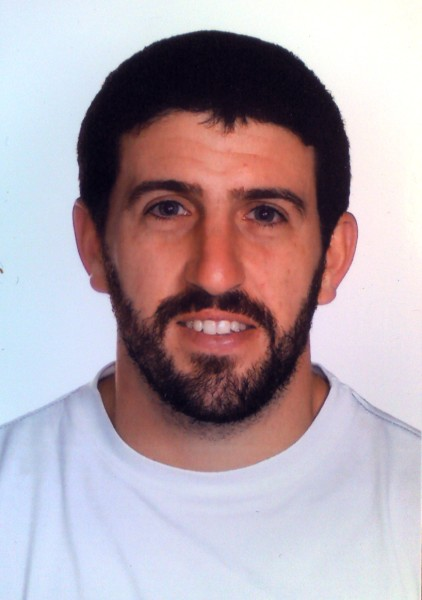
\includegraphics[bb=0 0 422 600,scale=0.2,keepaspectratio=true]{./gavila.jpg}
%  % gavila.jpg: 422x600 pixel, 72dpi, 14.89x21.17 cm, bb=0 0 422 600
% \end{figure}


\subsection*{Información Personal:}

%   \begin{wrapfigure}{l}{0.2\textwidth}
%   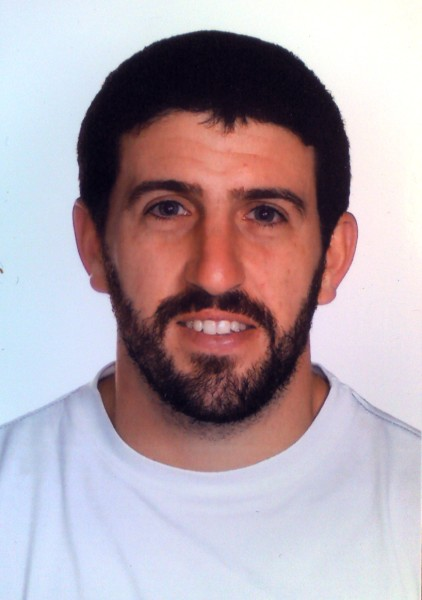
\includegraphics[height=3.5cm]{./gavila.jpg}
%   \end{wrapfigure}

\begin{tabular*}{0.1\textwidth}{@{\extracolsep{\fill}} l p{0.6\textwidth} }
\textbf{Fecha de nacimiento:} & 16 de Agosto, 1982\\
\textbf{Lugar de nacimiento:} & Córdoba Capital, Córdoba, Argentina\\
\textbf{Nacionalidades:} & Argentino, Italiano\\
\textbf{Direcci\'on Personal:} & 9 de Julio 2108 2do A,
X5002 Córdoba, Argentina\\
\textbf{Tel\'efono:} & +54 9351 2 055 880\\
\textbf{E-mail:} & \texttt{avila.gas@gmail.com}
\end{tabular*}

\vspace{1\baselineskip}
\HRule


\section{Formación académica}

\begin{itemize}
\item \textbf{Postgrado:} (28/11/2011) Doctor en Física.
Universidad de Potsdam, Alemania. Director: Prof. Dr. Helmut
Friedrich. Soporte económico y lugar de trabajo provistos por el Max Planck
Institute for Gravitational Physics (Albert Einstein Institute).

 \item \textbf{Universitaria:} (2002 - 2008) Licenciatura en Física, FaMAF,
Universidad Nacional de Córdoba, Argentina. Promedio general 9,57.
%Graduated on the 27/03/2008

 \item \textbf{Secundaria:} (1996 - 2001) Bachiller Técnico
Metal-Meácnico
especialista en Máquinas Herramienta, Instituto Técnico Renault, Córdoba,
Argentina. % Graduated with the highest average grade of the class of 2011.
\end{itemize}

\section{Experiencia docente}
\begin{itemize}
 \item(03/2010--09/2010) Asistente de trabajos prácticos: ``Theoretische
Physik: Mechanik I'', Prof. Dr. Achim Feldmeier. Potsdam University, Germany.
 \item(03/2007--03/2008) Ayudante alumno (cat. A). FaMAF, UNC, Argentina.
 \item(03/2005--03/2007) Ayudante alumno (cat. B). FaMAF, UNC, Argentina.
%  \item[01/2006--06/2007] Tutor and Supervisor, Online Tutor on College and
% Pre-college Matematics in English, Latinhire, Chile. (subcontracted Tutor.com)
\end{itemize}

\section{Conocimientos en informática}
\begin{itemize}
 \item Sistemas operativos: Linux (Ubuntu),
 \item Lenguajes: Python, JavaScript, SQL, Html5, CSS
 \item GIS y geolocalización: Internals de OpenStreetMap, JOSM, Merkaartor,
Maperitive, Mapnik, GeoJSON
 \item Client side Web: Backbone.js, Angular.js, Openlayers.js, Google Maps API 
v3, Require.js, Handlebars.js, Lodash.js
 \item Server side Web: Python WSGI (Flask), Node.js usando Express.js, 
RESTful APIs usando SWAGGER, Mongoose (Mongo), Passport (Authentication)
 \item Bases de datos: PostgreSQL, SQLite, mongoDB,
 \item Protocolos de datos públicos: General Transit Feed Specification (GTFS), 
GeoJSON, KML, GPX, OSM, GeoJSON, SHP
\end{itemize}

\section{Experiencia laboral}
\begin{itemize}
 \item (08/2014 -- presente) Sistemas Globales S. A., desarrollador web UI. 
  \subitem Virgin Mega: Lider técnico en proyecto hybrid angularjs + cordova para iPhone.
  \subitem Thomas Cook: Desarrollo fullstack javascript (BE: node.js, FE: backbone.js)

 \item (04/2014 -- presente) Ministerio de Transporte de la Provincia de Mendoza. Arquitectura 
 y desarrollo de applicacion de transporte público para publicacion de GTFS. 
 Aplicaciones web de geo-referencia, análisis de datos y modelos.

 \item (12/2011 -- 06/2014) Municipalidad de Córdoba, asesoramiento técnico en 
 Comisión de Movilidad Integral. Aplicaciones web de geo-referencia, análisis de
datos y modelos.

 \item (12/2012 -- presente) Desarrollo de aplicaciones web y asesoramiento 
 informático a empresas de transporte público. 

 \item (04/2008 -- 11/2011) Max Planck Institute for Gravitational Physics
(Albert Einstein Institute). PhD Candidate.
\end{itemize}

\section{Publicaciones}
\begin{enumerate}
\item \newblock \emph{Asymptotic staticity and tensor decompositions with fast
decay conditions}
\newblock (Disertación doctoral)
\newblock Dr. Gast\'{o}n~A Avila.
\newblock {Institutional Repository of the University of Potsdam},
\url{http://opus.kobv.de/ubp/volltexte/2011/5404/} 07.10.2011.
\item \newblock \emph{The Yamabe invariant for axially symmetric initial data of
two Kerr black holes.}
\newblock Gast\'{o}n~A Avila and Sergio Dain.
\newblock {Classical and Quantum Gravity},
\href{http://dx.doi.org/10.1088/0264-9381/25/22/225002}{25(22):225002 (13pp),
2008}.
\end{enumerate}

\section{Reconocimientos}
\begin{itemize}
 \item Graduado magna cum laude 2011, Universidad de Potsdam, Alemania.
 \item Abanderado de la promoci\'on 2001 - Instituto Técnico Renault,
 \item Premio a la exelencia académica 2001, Banco Roela, Argentina.
\end{itemize}

\section{Presentaciones en congresos}
\begin{itemize}
 \item \emph{Tensor decompositions with fast decay conditions at space-like
infinity}, Grav11 - FaMAF, Córdoba, Argentina. 11/04/2011.
 \item \emph{Tensor decompositions with fast decay conditions at space-like
infinity}, Workshop on Mathematical Relativity - ESI, Vienna, Austria.
28/01/2011.
 \item \emph{The Yamabe invariant for axially symmetric two Kerr black
holes initial data}, Grav09 - Córdoba Argentina. 15/04/2009.
\end{itemize}

\section{Reuniones cient\'ificas}
\begin{itemize}
 \item \emph{Grav11}, Congress on General Relativity and Gravitation (FaMAF),
La Cumbre, Córdoba, Argentina. 11/04/2011 - 15/04/2009. 
 \item \emph{Workshop on Mathematical Relativity}, International Centre for
Mathematical Science - Edinburgh, UK. 1/09/2009 - 7/09/2010.
 \item \emph{Seminar on Mathematical Relativity} - Erwin Schroedinger
Institute, Vienna, Austria. 27/01/2011 - 29/01/2011.
 \item \emph{Space, Time and Beyond}. Conference in honor of Helmut
Friedrich's birthday.
08/10/2009 - 09/10/2009.
 \item \emph{Grav09}, Congress on General Relativity and Gravitation, FaMAF,
Córdoba, Argentina. 13/04/2009 - 17/04/2009. 
%  \item \emph{Grav07}, Congress on General Relativity and Gravitation, FaMAF,
% Córdoba, Argentina. 5/11/2007 - 7/11/2007. %Asistent
 \item \emph{Grav06}, Fifty years of FaMAF \& Workshop on Global Problems in GR,
FaMAF, Córdoba, Argentina. 6/10/2006 - 11/10/2006. %Asistent
\end{itemize}

\section{Idiomas}
\begin{itemize}
%  \item \textbf{EsSpanish:} Native.
 \item \textbf{Ingl\'es:} Fluido
\end{itemize}


\vspace{2\baselineskip}

\begin{flushright}
\rule{7cm}{0.2mm}

 Córdoba,
 \today
\end{flushright}


\end{document}
